% Chapter Template

\chapter{Performance and Transferability of DBM: Reverse-mapping of Syndiotactic Polystyrene} % Main chapter title
\label{bm_ps} % Change X to a consecutive number; for referencing this chapter elsewhere, use \ref{ChapterX}

In this chapter, DBM is applied to a challenging condensed-phase molecular system that consists of syndiotactic polystyrene (sPS) polymers. The performance of DBM is analyzed in terms of three important aspects: 1) The general reverse-mapping capability of the model, i.e. the ability to reproduce a reference atomistic distribution from coarse-grained configurations. 2) The transferability of the model across different state points. To this end, DBM is trained solely on data obtained in a high-temperature melt and the model's transferability to lower temperatures is probed. 3) The transferability of DBM across chemical space. Here, DBM is trained on liquids of small molecules. After training, the model is deployed on the more challenging polymeric system of sPS. 

This chapter presents content that has been previously published in the following research articles. The content is reproduced here with kind permission from the other authors and the corresponding Journals published this work.

\hfill \break
\noindent \textit{Marc Stieffenhofer, Michael Wand, Tristan Bereau}\\
\textbf{Adversarial reverse mapping of equilibrated condensed-phase molecular structures}\\
Machine Learning: Science and Technology, Volume 1, Number 4\\
DOI: 10.1088/2632-2153/abb6d4\\
$\copyright$ IOP Publishing Ltd, 2020
\hfill \break

\noindent \textit{Marc Stieffenhofer, Tristan Bereau, Michael Wand}\\
\textbf{Adversarial reverse mapping of condensed-phase molecular structures: Chemical transferability}\\
APL Materials 9, Volume 9, Number 3\\
DOI: 10.1063/5.0039102\\
$\copyright$ AIP Publishing LLC, 2021
\hfill \break

\section{Set-up and Reference Data}

In this section, the reference data used to train and evaluate the performance of DBM is introduced. In addition, a baseline method is utilized to compare the backmapped results of DBM with a state-of-the-art method. 

\subsection{Syndiotactic Polystyrene}
\label{SEC:sPS}

\begin{figure}
  \centering
  \captionsetup{width=1.0\linewidth}
      \includegraphics[width=0.70\textwidth]{./Figures/adversarial_backmapping/intro.pdf}
  \caption{Coarse-grained and atomistic representation of sPS. The coarse-grained monomer consists of two beads, denoted $A$ for the chain backbone and $B$ for the phenyl ring. \cite{stieffenhofer2020adversarial}}
  \label{FIG:sPS_single_chain}
\end{figure}

Polystyrene (PS) is an aromatic polymer made from the monomers styrene, which is an organic compound consisting entirely of carbon and hydrogen. Physical and chemical properties of PS depend significantly on its tacticity, i.e. the arrangement of the phenyl groups along the polymer backbone. In this study, syndiotactic polystyrene (sPS) is used, where the phenyl groups are arranged on alternating sides of the polymer backbone. An illustration of a single polymer chain with atomistic as well as coarse-grained resolution is shown in Fig. \ref{FIG:sPS_single_chain}. 

Despite its simple chemical structure, sPS displays a rich conformational space and exhibits complex polymorphic behavior. As such, sPS is a well suited candidate to study the transferability properties of DBM. Upon thermal annealing, a sPS melt undergoes a phase transition from amorphous to a crystalline phase at $T \approx 450$ K.\cite{liu2018polymorphism} Five different crystalline forms of sPS have been reported experimentally. Here, the focus is set on the $\alpha$ and $\beta$ polymorphs, which are illustrated in Fig. \ref{FIG:sPS_polymorphs}.

The atomistic data in this study is reported in Liu \emph{et al.};\cite{liu2018polymorphism} the underlying force field is based on the work of Mueller-Plathe.\cite{muller1996local} The system is sampled using Replica Exchange MD simulations, which are performed using the molecular dynamics package {\sc GROMACS} 4.6.\cite{hess2008gromacs} The simulations are carried out in the NPT ensemble using the velocity rescaling thermostat and the Parrinello-Rahman barostat. An integration time step of $1$ fs is used. For additional details regarding the simulations the reader is referred to the work of Liu \emph{et al.}\cite{liu2018polymorphism}

Pairs of corresponding fine- and coarse-grained snapshots are generated by mapping atomistic configurations onto the coarse-grained resolution. Three data sets are constructed from uncorrelated snapshots selected from different trajectories simulated at $T = 313$ K, $453$ K, and $568$ K. To cover a wide range of conformational space, each atomistic simulation was initialized from a different structure: The simulation at $313$ K started from a $\beta$ structure, at $453$ K from an $\alpha$ structure and at $568$ K from an amorphous configuration. The system includes $36$ polystyrene chains and each chain consists of $10$ monomers. Each data set contains $12$ snapshots for training and $78$ snapshots for testing.

The fine-to-coarse mapping is based on the coarse-grained model developed by Fritz \emph{et al.}.\cite{fritz2009coarse} Each monomer is mapped onto two beads of different types, denoted $A$ for the chain backbone and $B$ for the phenyl ring (see Fig. \ref{FIG:sPS_single_chain}). Bonds are formed only between backbone and phenyl ring beads $A$-$B$, i.e. the coarse-grained polymer is represented as a linear chain. The coarse grained model, parameterized in the melt, is transferable to the crystalline phase and stabilizes the experimentally observed $\alpha$ and $\beta$ polymorphs. 

%In isotactic PS the phenyl groups are positioned on the same side of the polymer chain, while in syndiotactic PS the phenyl groups are arranged on alternating sides of the chain. In atactic PS the phenyl groups are arranged randomly. 

\subsection{Octane and Cumene}
\label{SEC:Oct_Cum}

Octane and cumene are small hydrocarbons. While octane is an acyclic alkane, cumene is aromatic. MD simulations of octane ad cumene liquids are performed using the molecular dynamics package {\sc GROMACS} 5.0.\cite{hess2008gromacs} The GROMOS force-field is used and topologies are generated by {\sc Automated Topology builder}.\cite{malde2011automated} Note that the GROMOS and sPS force fields differ in parameterization strategies. While both force-fields aim at reproducing thermodynamic properties, the GROMOS force-field is designed for a broad range of chemistries, while the parametrization for sPS is custom-built from a specific force field designed for benzene. This leads to evident differences in force-field parameters, especially in terms of the non-bonded Lennard-Jones interaction and partial charges.

The simulation boxes of octane and cumene contain 215 and 265 molecules, respectively. MD simulations are performed in the NPT ensemble using the velocity rescaling thermostat and the Parrinello–Rahman barostat. The integration time step of is set to 1 fs and both systems are sampled at $350$ K.

As illustrated in Fig. \ref{FIG:cheh_trans_intro}, the fine-to-coarse mapping is based on the mapping for sPS. Cumene is mapped onto one bead of type $B$ for the phenyl ring and two beads of type $A$ for the backbone, each containing a methyl group and sharing the $CH$ group connected to the phenyl ring. Octane is mapped onto four beads of type $A$, where neighboring $A$ beads share a $CH_{2}$ group.

\subsection{Baseline method}

The results of DBM are compared to a generic backmapping strategy, as described in Sec. \ref{SEC:bm_generic}. Specifically, the backmapping script developed by Wassenaar \emph{et al.} is utilized.\cite{wassenaar2014going} In a first step, this method places each particle on the weighted average position of the coarse-grained beads it corresponds to and optionally adds a random displacement. In addition, the protocol allows to apply geometric modifiers setting the alignment of the next particle cis, trans, out, or chiral with respect to the other particles. The modifiers are crucial for the performance of this method and require a careful construction by the user.

After the initial structure is generated, the protocol by Waasenaar \emph{et al.} continues with multiple cycles of force-field based energy minimization for relaxation. Here, the first cycle consists of $200$ steps and is performed without non-bonded interactions. Afterwards, all interactions are turned on and energy minimization continues with a total number of $5000$ steps. The original protocol continues with several cycles of position restrained MD simulations to equilibrate the relaxed system. However, comparing DBM with such equilibrated structures is pointless, since applying MD simulations would obviously reproduce the correct Boltzmann distribution. DBM aims at generating molecular structures without relying on further MD simulations. Therefore, the script by Waasenaar \emph{et al.} is stopped after the relaxation to allow for a more stringent comparison.

\subsection{Specifications of DBM}

DBM deploys a convolutional neural network (CNN) architecture with residual connections for the generator $g_{\Theta}$ and critic $c_{\Psi}$.\cite{he2016deep} A detailed description of the network architecture can be found in Fig. \ref{APPENDIX:DBM_architecture}. Training is performed using the Adam optimizer.\cite{kingma2014adam} To prevent numerical instabilities in the beginning of the training, the prefactor for the regularization term based on the potential energy is set initially to $\lambda_{\text{pot}}= 0$ and increased smoothly to $\lambda_{\text{pot}} = 0.01$. The prefactor scaling the weight of the gradient penalty term is set to $\lambda_\textup{gp} = 0.1$ throughout the training. To obtain reliable gradients for the generator, the critic $c_{\Psi}$ is trained five times in each iteration while the generator $g_{\Theta}$ is trained once.

The autoregressive approach of DBM is prone to accumulate errors, i.e. misplaced atoms can hinder $g_{\Theta}$ to find suitable positions for subsequent atoms. As a remedy, the potential energy is used during inference in order to spot and reject outliers. In particular, a mini-batch is constructed for each structure that displays it at various different relative orientations around the director axis (see Sec. \ref{DBM:loc_env}). Since the CNN architecture is not rotational equivariant, predictions will slightly differ depending on the chosen orientation. As a straight-forward solution to remove outliers, the structure with the lowest potential energy is selected from the generated ensemble. In addition, hydrogens are removed from the current and adjacent beads for the reconstruction of heavy atoms, such that misplaced hydrogens don't affect the positioning of heavy atoms.

\section{General Performance}
\label{SEC:DBM_general_performance}

At first, the general performance of DBM is probed. To this end, DBM is trained on the high-temperature, amorphous data set at $568$ K. After training, the model is deployed to test data, i.e. hold-out data at the same temperature.   

\subsection{Results}

\begin{figure}
  \centering
  \captionsetup{width=1.0\linewidth}
      \includegraphics[width=1.05\textwidth]{./Figures/adversarial_backmapping/sPS_temp_trans/ff_dists_and_rdf.pdf}
  \caption{ Canonical distributions for various force-field interaction terms at (left) $T$ = 568 K, (middle) $T$ = 453 K and (right) $T$ = 313 K for reference structures (black), structures generated with the baseline, energy-minimization-based backmapping method (red), and the new method DBM (blue). The model is trained solely on the high temperature data (left), but deployed at lower temperatures (middle and right). (a)–(c) C-C-C backbone angle, (d)–(f) C-C-C-C backbone dihedral, (g)–(i) C-C-C-C improper dihedral, (j)–(l) Lennard-Jones energies, and (m)–(o) radial distribution functions, g(r), of the non-bonded carbon atoms.\cite{stieffenhofer2020adversarial}}
  \label{FIG:sPS_temp_trans_ff_dists}
\end{figure}

Fig. \ref{FIG:sPS_temp_trans_ff_dists} displays distribution functions for several structural and energetic properties of sPS. The distributions of intramolecular carbon backbone angle and dihedral, shown in FIG. \ref{FIG:sPS_temp_trans_ff_dists} (a) and (d), are in excellent agreement with the reference distributions. On the other hand, structures generated with the baseline method show too narrow distributions, which is expectable from an approach based on energy minimization. As shown in Fig. \ref{FIG:sPS_temp_trans_ff_dists} (g), the distribution for the carbon improper dihedral of the phenyl group is slightly too narrow for configurations generated with DBM. However, the small range of angles due to the imposed planarity of the ring has to be emphasized. The distribution of the baseline method is even more peaked, i.e. fluctuations around the planar structure are significantly suppressed.

A very important aspect towards generating well-equilibrated configurations in a condensed environment is the correct reproduction of Lennard-Jones energies. Fig. \ref{FIG:sPS_temp_trans_ff_dists} (j) displays the distribution of Lennard-Jones energies obtained for each chain separately. While structures generated with DBM show slightly too large high-energy tails, the overall match with the reference distribution is remarkably good. On the other hand, the baseline method systematically and drastically over-stabilizes the system. 

Further, the radial distribution function is analyzed to probe the ability of DBM to reproduce large-scale structural features. Fig. \ref{FIG:sPS_temp_trans_ff_dists} (m) displays the pair correlation function $g(r)$ for non-bonded carbon pairs. Structures generated with DBM show an excellent agreement with the reference distribution indicating that the local packing of the polymer chains is well reproduced. The baseline method is not able to reproduce the pair correlation correctly.

\subsection{Discussion}

DBM is an ML approach for the backmapping of coarse-grained molecular structures. The DNN based model learns to reproduce local features guided by large-scale structures from a coarse-grained snapshot. Here, it is applied to the high-temperature data set of an complex condensed-phase molecular system made of sPS chains. The results are compared with a baseline method based on energy-minimization.

It is shown that he method reproduces structural and energetic properties of the reference system remarkably well. DBM yields well-equilibrated configurations of a Boltzmann distribution at a state point it was trained on. On the other hand, the baseline method based on energy minimization over-stabilizes the system. As such, it does not account for the diversity of microstates at a specific canonical state point. Consequently, further MD simulations controlled by a thermostat would be required to recover the correct state point.

\section{Temperature Transferability: From Melt to Crystal}
\label{DBM:temp_trans}

After successfully recovering the state point DBM was trained on, the model's ability to transfer across temperatures is probed. As illustrated in Fig. \ref{FIG:sPS_polymorphs}, the training of DBM is fixed to the high-temperature ensemble, while testing is performed at lower temperatures \textit{without} reparameterization. Specifically, the model is trained at $568$ K and tested at $453$ K and $313$ K. Importantly, the sPS system undergoes a phase transition at $\approx 450$ K, going from an amorphous phase to a crystalline state with different polymorphs. As such, the test data sets not only differ in terms of temperature compared to the training data set, but also display different state points, i.e. the $\alpha$ and $\beta$ polymorphs. 

\begin{figure}
  \centering
      \includegraphics[width=0.6\textwidth]{./Figures/adversarial_backmapping/sPS_temp_trans/ps_polymorphs.pdf}
  \caption{Polymorphism of Polystyrene. At high temperature ($T$ = 568 K) the system stabilizes an amorphous phase. At lower temperatures the CG model mostly stabilizes the $\alpha$ polymorph at $T$ = 453 K and the $\beta$ polymorph at $T$ = 313 K. DeepBackmap is trained solely on the high-temperature ensemble ($T$ = 568 K) and test its transferability to the lower temperatures. \cite{stieffenhofer2020adversarial}}
  \label{FIG:sPS_polymorphs}
\end{figure}

\subsection{Results}
\label{DBM:sPS_temp_trans}

As shown in Fig. \ref{FIG:sPS_temp_trans_ff_dists} (middle and right culumn), the distributions of structural and energetic features display a number of significant changes upon cooling: distributions of angles become narrower, the side peak in the backbone dihedral vanishes, the distributions of Lennard-Jones energies are shifted towards lower energies and the pair correlation of non-bonded carbon atoms is more peaked. 

\subsubsection{Distributions of Structural and Energetic Features}

DBM adapts remarkably well to the crystalline state points. Fig. \ref{FIG:sPS_temp_trans_ff_dists} (b,c,e,f,h,i) indicate that the angle and dihedral distributions for structures generated with DBM follow the reference distributions and become narrower. Lennard-Jones energies displayed in Fig. \ref{FIG:sPS_temp_trans_ff_dists} (k,l) are also shifted and match with the reference distributions. Moreover, the local packing of the sPS chains is perfectly reproduced even in the crystalline phase, as indicated in Fig. \ref{FIG:sPS_temp_trans_ff_dists} (n,o). 

On the other hand, the baseline method does not adapt well to lower temperatures. The method based on energy minimization is not able to generate the correct features at the crystalline state points, but retains much of its features found at high temperature. This becomes especially apparent for the side peak of the backbone dihedral and the flat pair correlation function $g(r)$.

\subsubsection{Sketch-Map}

\begin{figure}[h]
  \centering
      \includegraphics[width=1.0\textwidth]{./Figures/adversarial_backmapping/sPS_temp_trans/sm_snapshots.pdf}
  \caption{ Low-dimensional structural space of condensed-phase configurations at (a) $T$ = 568 K, (b) $T$ = 453K and (c) $T$ = 313 K. For each panel, snapshots are backmapped from identical coarse-grained configurations, highlighting the overlap between reference and DeepBackmap, but disconnect from the baseline method.\cite{stieffenhofer2020adversarial}}
  \label{FIG:sPS_temp_trans_SM}
\end{figure}

Evaluating large-scale structural features beyond pair-statistics is challenging, since the high dimensionality of the system does not allow to directly visualize the configuration space. For this reason, dimensionality reduction is applied to further examine the model's accuracy at higher order. As explained in Sec. \ref{MS:sketchmap}, linear dimensionality reduction techniques are insufficient in many cases to capture the global structure of data obtained from MD trajectories. Therefore, Sketch-Map (SM) is applied to build a two-dimensional map representing proximity relationships between sPS chains.\cite{ceriotti2011simplifying, tribello2012using}

The descriptors for the sPS chains consist of a set of representations for the local environments $\mathcal{H}$ centered around alternating backbone carbon atoms that are directly linked to a phenyl group. The pairwise distance between two such environments is encoded using a similarity kernel $k(\mathcal{H}, \mathcal{H}') = \mathbf{p}(\mathcal{H}) \mathbf{p}(\mathcal{H'})$ based on the normalized many-body smooth overlap of atomic position (SOAP) representation $\mathbf{p}(\mathcal{H})$.\cite{bartok2013representing} Hydrogen atoms are neglected in the SOAP representation. To compare two sPS chains $a$ and $b$, the covariance matrix 

\begin{equation}
 C_{ij}(a,b) = \mathbf{p}(\mathcal{H}^a_i) \mathbf{p}(\mathcal{H}^b_j)
\end{equation}

is computed, which contains the complete information of the pairwise similarity of all local environments taken into account between the two structures. In order to obtain a global similarity kernel $k(a,b)$, the covariance matrix $C_{ij}(a,b)$ has to be mapped to a single scalar value, which is achieved using a regularized entropy match kernel.\cite{de2016comparing}

Fig. \ref{FIG:sPS_temp_trans_SM} displays the obtained two-dimensional map, where each point represents a single sPS polymer chain. A number of clusters is shown that correspond to different environments. The reference data (black) shows a single cluster for the low-temperature data at $313$ K (Fig. \ref{FIG:sPS_temp_trans_SM} (c)) corresponding to the $\beta$ polymorph. The high-temperature data at $568$ K (Fig. \ref{FIG:sPS_temp_trans_SM} (a)) is mapped to multiple clusters indicating more diversity, i.e. it includes amorphous, $\alpha$ and other structures. The data set at an intermediate temperature $453$ K (Fig. \ref{FIG:sPS_temp_trans_SM} (b)) shows less diversity and is mapped mostly to the cluster corresponding to the $\alpha$ polymorph, but still contains some amorphous and other structures.

Structures obtained with DBM (blue) overlap significantly with the reference points for all three data sets indicating closeness in configuration space and high fidelity of the backmapped structures. This is in strong contrast to the energy-minimized structures obtained with the baseline method, which cover different areas in the two-dimensional projection of configuration space. Moreover, the baseline method fails to recover the correct number of clusters for all three temperatures highlighting a lack of temperature sensitivity.

\subsubsection{MD Simulation}

Backmapped structures that serve as a starting point for further MD simulations typically require lengthy preparations, such as energy minimization, temperature ramp up phase and thermostat/barostat equilibration. Here, the high quality of backmapped structures obtained with DBM is highlighted by running MD simulations \textit{without} any heat-up.

The simulations are carried out in the NPT ensemble using the velocity rescaling thermostat and the Parrinello-Rahman barostat. Initial velocities are generated according to a Maxwell distribution and an integration timestep of $1$ fs is used. 

Fig. \ref{FIG:sPS_eq} displays the time evolution of the potential energy during the simulations at (a) $T = 313$ K and (b) $T = 568$ K. Simulations starting from reference or backmapped structures obtained with DBM show a similar evolution of the potential energy at both temperatures and reach a steady value after $\approx 100$ ps. On the other hand, simulations starting from backmapped structures obtained with the baseline method show a different behaviour. The potential energy of simulations performed at $313$ K settles at significantly higher energies compared to reference and DBM structures. This indicates badly initialized structures that get trapped into local minima with high energy barriers. However, this issue is not apparent anymore at $568$ K and all simulations show a similar behaviour independent of their initialization. This can be rationalized with the high temperature that allows to escape local minima with higher probability. 

\begin{figure}
  \centering
  \captionsetup{width=1.0\linewidth}
      \includegraphics[width=1.0\textwidth]{./Figures/adversarial_backmapping/sPS_temp_trans/eq.pdf}
  \caption{Evolution of the potential energy in MD simulations without heat-up starting from reference structures (black), backmapped structures obtained with the baseline method (red) and backmapped structures obtained with DBM (blue).\cite{stieffenhofer2020adversarial}}
  \label{FIG:sPS_eq}
\end{figure}

\subsection{Discussion}

In this section, the temperature transferability of DBM is probed. While training of the model is fixed to melt configurations at high temperature, it is deployed at lower temperatures, where the sPS system is in a crystalline state. However, DBM retains its performance displayed in Sec. \ref{SEC:DBM_general_performance} and reproduces the reference distributions with remarkable accuracy. In addition, a higher-order investigation, facilitated by the Sketchmap algorithm, emphasizes the high structural fidelity. As such, the model learns to reproduce local correlations that are transferable across different state points. This is in strong contrast to the baseline method, which lacks accuracy and temperature sensitivity. 

These remarkable transferability features of DBM can be rationalized in terms of a scale-separation: The model learns to reproduce well-equilibrated local correlations while large-scale features are dictated by the coarse-grained snapshot. As such, the backmapped structure is composed of two sources of information, i.e. 1) the learned local features and 2) the coarse-grained structure. However, most of the temperature dependence is carried by the latter, as it is shown by Liu \emph{et al.} that the applied coarse-grained model reproduces the crystallization transition remarkably well. On the other hand, local features are less temperature sensitive, since they correspond primarily to covalent interactions that operate on energy scales significantly larger than $k_B T$. As such, the local correlations learned in the melt are transferable across a phase transition. However, it is not clear whether the other direction, i.e. training at low temperature and transferring to higher temperatures, would yield satisfactory results, because of the broader conformational space spanned at higher temperatures.

\section{Chemical Transferability: From Small Molecules to Polymers}

In this section, the transferability of DBM across chemical space is explored. To this end, the generalization of the model beyond the chemistry used for training is probed by recycling the learned local correlations to make predictions for molecules absent from the training data set. 

DBM uses an sequential approach to reconstructs atomic environments. Further, it is based on the locality assumption, i.e. the placement of one atom is assumed to rely only on short-range force-field related features. As such, DBM only learns local correlations while large-scale features are adapted from the coarse-grained structure. It can be hypothesized that such local environments strongly overlap across chemical space, and thus, it is likely that small-scale features can be shared between different molecules. This makes DBM a promising candidate toward achieving chemical transferability. 

\begin{figure}
  \centering
  \captionsetup{width=1.0\linewidth}
      \includegraphics[width=1.0\textwidth]{./Figures/adversarial_backmapping/sPS_chem_trans/intro.pdf}
  \caption{All-atom and coarse-grained representations of different molecules. A similar coarse-to-fine mapping is used for all molecules (beads denoted $A$ for the chain backbone and $B$ for the phenyl ring). The chemical transferability of DBM is probed by training it solely on octane and cumene structures and then apply it to the more challenging system of syndiotactic polystyrene.\cite{stieffenhofer2020adversarial}}
  \label{FIG:cheh_trans_intro}
\end{figure}

The model is trained on molecular liquids of octane and cumene molecules. After training, the model is reused for a more complex polymeric system consisting of sPS molecules. While sPS shares some features with cumene and octane, it is still sufficiently complex to study the limitations of the generalization. As such, the pertinent but imperfect match between the small molecules and polymer offers a stringent backmapping exercise.

In addition, the role of the different types of force-field based regularization introduced in Sec. \ref{SEC:DBM_regularization} is explored by comparing their impact on the performance of the model, especially regarding chemical transferability.


\subsection{Results}

The training set contains 3225 and 2120 molecules of octane and cumene in the liquid state, respectively. After training, DBM is applied to a test set consisting of 720 chains (7200 monomers) of sPS melt. While octane and cumene liquids are simulated at $T = 350$ K, the sPS melt is simulated at $T = 568$ K. The discrepancy in the temperature for the training and test sets is a consequence of the different boiling and melting points of the molecules, as the model's transferability shall be probed in the liquid state. However, as shown in Sec. \ref{DBM:temp_trans}, the learned local correlations are weakly sensitive to changes in the temperature.

\subsubsection{Distributions of Structural and Energetic Features}

Fig. \ref{FIG:sPS_chem_trans_angles}-\ref{FIG:sPS_chem_trans_nb} display various distribution functions for structural and energetic properties of sPS derived for reference structures and structures generated with DBM. Three different regularization configurations are applied for the training of the model: Either $\mathcal{C}_1$ ("energy minimizing") or $\mathcal{C}_2$ ("energy matching") terms are added to the cost-function of the generator, as explained in Sec. \ref{SEC:DBM_regularization}, or no regularization is used. Results are shown for the chemically specific models, i.e. trained directly on sPS (left), and chemically transferred models, i.e., trained solely on octane and cumene configurations (right).

\begin{figure}
  \centering
  \captionsetup{width=1.0\linewidth}
      \includegraphics[width=1.05\textwidth]{./Figures/adversarial_backmapping/sPS_chem_trans/angles.pdf}
  \caption{Canonical distributions for sPS at $T = 568$ K. (a)-(h) Various angle terms for reference structures and structures generated with DBM using different regularization terms during training are shown. Left: Chemically specific models trained on the sPS liquid at $T = 568$ K. Right: Chemically transferred models trained on octane and cumene liquids at $T = 350$ K.\cite{stieffenhofer2020adversarial}}
  \label{FIG:sPS_chem_trans_angles}
\end{figure}

Fig. \ref{FIG:sPS_chem_trans_angles} shows different angle distributions. The general performance of chemically-transferred models is mixed and deviates from the chemically-specific models. The largest discrepancy can be found for the carbon backbone angle displayed in panel (a) and (b). While models trained directly on sPS reproduce the angles of the carbon chain with remarkable accuracy, models trained on cumene and octane generate structures with overly broad distributions. However, the overall accuracy of further angles (panels (c) - (h)) reproduced by the chemically-transferred models is exceedingly satisfactory. They even outperform the chemically-specific models, which yield distributions that are slightly too narrow. The role of the regularization applied during training is not significant.

\begin{figure}
  \centering
  \captionsetup{width=1.0\linewidth}
      \includegraphics[width=1.05\textwidth]{./Figures/adversarial_backmapping/sPS_chem_trans/dihs.pdf}
  \caption{Canonical distributions for sPS at $T = 568$ K. Various dihedral terms for reference structures and structures generated with DBM using different regularization terms during training are shown. (a), (b), (e), and (f) Proper dihedral; (c), (d), (g), and (h) improper dihedral. Left: Chemically specific models trained on the sPS liquid at $T = 568$ K. Right: Chemically transferred models trained on octane and cumene liquids at $T = 350$ K.\cite{stieffenhofer2020adversarial}}
  \label{FIG:sPS_chem_trans_dihs}
\end{figure}

Next, the distributions of various dihedral distributions are displayed in Fig. \ref{FIG:sPS_chem_trans_angles}. Again, the accuracy of chemically-transferred models is mixed compared to chemically-specific models. All models are able to reproduce the planarity of the ring with high accuracy, as displayed in panels (c)-(d) and (g)-(h). While the distributions for the improper dihedrals are slightly too narrow compared to the reference, the small range of the distribution has to be emphasized. However, the models trained directly on sPS outperform the chemically-transferred models in terms of the accuracy of the backbone dihedrals shown in panels (a)-(b) and (e)-(f). The chemically-specific models fail to reproduce the height of the main peak and are not able to reproduce the side peak of the proper backbone dihedral. Similarly, both peaks in the distribution of the C-C-C-H backbone dihedral are too broad. The configuration of the regularization again has no impact on the observed distributions. 

\begin{table}
\begin{tabular}{ c|c|c } 
distribution & chemically-specific & chemically-transferred \\
\hline
angle backbone& 0.0183 & 0.2144 \\ 
angle phenyl ring& 0.1084 & 0.0305 \\ 
proper dihedral backbone& 0.0196 & 0.1214 \\ 
improper dihedral phenyl ring& 0.1898 & 0.0783 \\ 
\caption{ Jenson-Shannon divergence of reference and backmapped distributions using either a chemically specific or chemically transferred model. Angle and dihedral distributions of the carbon backbone and phenyl ring of sPS are displayed. Models used this analysis are trained without regularization.}
\label{TAB:sPS_chem_trans}
\end{tabular}
\end{table}

Table \ref{TAB:sPS_chem_trans} reports Jenson-Shannon divergences between reference and backmapped distributions for a further comparison of the chemically-specific and the chemically-transferred models. The Jenson-Shannon divergences are computed for the carbon angles and dihedrals of the backbone and the phenyl ring of sPS. While the absolute values of the JS divergences are not informative, since they are sensitive to the specific bin size, they confirm the presumption made earlier: Chemically-transferred models lack the accuracy of the chemically-specific models in terms of the backbone structure but are able to reproduce aromatic rings with high accuracy.

\begin{figure}
  \centering
  \captionsetup{width=1.0\linewidth}
      \includegraphics[width=1.05\textwidth]{./Figures/adversarial_backmapping/sPS_chem_trans/non_bonded.pdf}
  \caption{Canonical distributions for sPS at $T = 568$ K. Lennard-Jones energies for all atoms (a) and (b), Lennard-Jones energies for carbon atoms (c) and (d), and radial distribution functions, $g(r)$, of the non-bonded carbon atoms (e) and (f) for reference structures and structures generated with DBM using different regularizations during training are shown. Left: Chemically specific model trained on the sPS liquid at $T = 568$ K. Right: Chemically transferred model trained on octane and cumene liquids at $T = 350$ K.\cite{stieffenhofer2020adversarial}}
  \label{FIG:sPS_chem_trans_nb}
\end{figure}

The ramification of the applied regularization during training becomes most evident in the distribution of the Lennard-Jones energies obtained for each sPS chain separately, which are displayed in Fig. \ref{FIG:sPS_chem_trans_nb} (a)-(d). Chemically specific models trained with regularization $\mathcal{C}^{(2)}_{\text{pot}}$ or without regularization reproduce the reference Lennard-Jones energies with high accuracy. Carbon-only Lennard-Jones energies match the reference distribution almost perfectly. However,  Lennard-Jones energies taking hydrogens into account show slightly too large high-energy tails for the backmapped structures. In contrast, applying regularization $\mathcal{C}^{(1)}_{\text{pot}}$ over-stabilizes the system and yields a significant shift of the distribution towards lower energies. However, these observations turn around for the chemically-transferred models: Here, regularization $\mathcal{C}^{(1)}_{\text{pot}}$ improves the performance dramatically compared to models trained with $\mathcal{C}^{(2)}_{\text{pot}}$ or without regularization. While the chemically-transferred model trained with $\mathcal{C}^{(1)}_{\text{pot}}$ reproduces the Lennard-Jones energies remarkably well except for high-energy tails, the other models yield backmapped structures with systematically too large Lennard-Jones energies.

The pair correlation function, $g(r)$, obtained for pairs of non-bonded carbon atoms is shown in Fig. \ref{FIG:sPS_chem_trans_nb} (e)-(f). All models are able to reproduce the pair correlation with high accuracy indicating a good agreement of the local packing of sPS chains with the reference structures.

\subsubsection{Sketch-Map}

Similarly to the previous evaluation, the accuracy of backmapped structures shall be probed at higher order deploying the SM algorithm, as described in \ref{MS:sketchmap} and \ref{DBM:temp_trans}. Specifically, local environments of sPS monomers are centered at backbone carbons that are connected with the phenyl group. The environments are encoded and compared using the SOAP representation, which yields a $N \times N$ similarity matrix for $N$ monomers. SM is applied to project this high dimensional representation of conformational space onto a two-dimensional embedding representing proximity relationships.

Fig. \ref{FIG:sPS_chem_tran_sm} (a) displays the obtained embedding for reference structures. $720$ landmarks (gray) are generated upon optimizing the SM cost-function in Eq. \ref{ML:SM_costfunction}. Afterwards, further $1440$ local environments are projected (black) into the SM space guided by the landmarks. Fig. \ref{FIG:sPS_chem_tran_sm} (b) shows the projections of backmapped structures obtained with a chemically-specific model (blue) and a chemically-transferred model (red). The underlying coarse-grained structures correspond to the atomistic structures used for the projections of reference structures in Fig. \ref{FIG:sPS_chem_tran_sm} (a). Both models are trained with $\mathcal{C}^{(1)}_{\text{pot}}$. Further plots for models trained with $\mathcal{C}^{(2)}_{\text{pot}}$ or without regularization can be found in Fig. \ref{APPENDIX:sm_p2_and_no_p} in the appendix. The high structural fidelity of both, the chemically-specific and the chemically-transferred model, is highlighted by the strong overlap of the projections obtained for reference and backmapped structures.

\begin{figure}
  \centering
  \captionsetup{width=1.0\linewidth}
      \includegraphics[width=1.05\textwidth]{./Figures/adversarial_backmapping/sPS_chem_trans/sm_ref_p1.pdf}
  \caption{Low-dimensional representation of condensed-phase configurations at $T = 568$ K. For each panel, snapshots are backmapped from identical coarse-grained configurations, highlighting the overlap between reference and DBM structures. (a) Landmarks and projections of reference structures and the obtained cluster centers. (b) Landmarks of reference structures and projections of structures generated with chemically-specific (red) and chemically-transferred (blue) models trained with $\mathcal{C}^{(1)}_{\text{pot}}$.\cite{stieffenhofer2020adversarial}}
  \label{FIG:sPS_chem_tran_sm}
\end{figure}

The two dimensional representations obtained with the SM algorithm form a number of distinct clusters. As such, points assigned to the same cluster indicate closeness in conformational space. For a further analysis, cluster centers are identified using the k-means algorithm. Each monomer embedding is assigned to the closest cluster. This yields a confusion matrix that allows to compare the cluster assignment of reference and backmapped structures. While the diagonal elements of the confusion matrix hereby refers to reference and backmapped structures that get mapped onto the same cluster, off-diagonal elements indicate a change of the cluster assignment upon coarse-graining and backmapping. The results for chemically-specific and chemically-transferred models trained with different regularization configurations can be found in Fig. \ref{FIG:sPS_chem_trans_hm}. Interestingly, the confusion matrix becomes most diagonal for models trained without regularization displayed in panels (c) and (g), respectively. However, the reduced resolution of the coarse-grained conformational space implies that an ensemble of microstates is associated with a single coarse-grained structure, as described in Sec. \ref{theory_backmapping}. The ensemble of microstates associated with the same coarse-grained structure might span a broad region in conformational space, which is not guaranteed to map onto the same cluster. As such, the diagonality of the confusion matrix is not necessarily a proper indicator for the quality of the backmapped distribution. More importantly, the relative populations of the clusters have to be reproduced, as this implies an accurate coverage of conformational space. Results comparing the relative cluster populations can be found below each confusion matrix in Fig. \ref{FIG:sPS_chem_trans_hm}. Chemically-specific models trained with $\mathcal{C}^{(2)}_{\text{pot}}$ or without regularization yield an excellent match of the relative populations. On the other hand, all chemically-transferred models lead to comparable accuracy independent of the regularization configuration: None of the chemically-transferred models reproduce the relative populations accurately.

\begin{figure}
\hspace*{-1cm}
  \centering
  \captionsetup{width=1.0\linewidth}
      \includegraphics[width=1.2\textwidth]{./Figures/adversarial_backmapping/sPS_chem_trans/hm.pdf}
  \caption{(Top) Confusion matrix for the different clusters obtained in the two-dimensional Sketchmap. (Bottom) Relative populations of the clusters. (a)–(c) chemically-specific models trained with (a) $\mathcal{C}^{(1)}_{\text{pot}}$, (b) $\mathcal{C}^{(2)}_{\text{pot}}$, and (c) no regularization. (d)–(f) chemically-transferred models trained with (d) $\mathcal{C}^{(1)}_{\text{pot}}$, (e) $\mathcal{C}^{(2)}_{\text{pot}}$, and (f) no regularization. “ol” refers to the outlier.\cite{stieffenhofer2020adversarial}}
  \label{FIG:sPS_chem_trans_hm}
\end{figure}

\subsection{Discussion}

In this section, the chemical transferability of DBM is probed. To this end, models trained solely on liquids of small molecules, i.e. octane and cumene, are deployed on the more complex polymeric system of sPS melts. The performance of such chemically-transferred models is compared with chemically-specific models, i.e. models trained directly on sPS. In addition, the role of the regularization applied during training is investigated.
The observed overall accuracy of chemically-transferred models is encouraging. The evaluation of structural distributions reveals the high quality of reconstructed phenyl groups. However, discrepancies in terms of the sPS backbone are discovered as well, i.e. carbon angle and dihedral distributions in the backbone have lower quality compared to chemically-specific models. On the other hand, chemically-transferred models retain their capability to reproduce non-bonded features in the challenging condensed-phase environment. They are able to recover the distribution of Lennard-Jones energies with remarkable accuracy and match the pair correlation function of the reference distribution virtually identically. The high structural fidelity of backmapped structures is also highlighted by a higher-order investigation facilitated by the SM algorithm. Although backmapped structures and their reference counterparts are not necessarily mapped onto the same cluster, as indicated by the confusion matrix, the correct spots in the two-dimensional projection of conformational space are covered. However, discrepancies in the relative statistical weight of reference and backmapped microstates are observed.

The performance of chemically-transferred models underpin the assumption that local chemical features are shared between molecules. It further highlights the capability of DBM to interpolate across these parts of chemical space due to its locality and sequential reconstruction. Specifically, the local correlations learned from octane and cumene liquids transfer to a great extend to sPS melts. However, the limits of generalization are shown as well, indicated by the limited quality of the reconstructed carbon backbone. It can be hypothesized that accuracy bottlenecks arise from missing features. In particular, local environments of backbone carbons connecting monomers are absent in the training examples. As such, training on an increasing number of building blocks should systematically improve the transferability of the backmapping procedure. Another important aspect affecting the transferability of DBM in this study are the force-field inconsistencies between the molecules. Therefore, conformational spaces are evidently incoherent and features found for fragments of sPS and cumene/octane are more dissimilar than first expected.

The applied regularization has marginal impact on the distributions associated with covalent interactions. However, distributions for the non-bonded Lennard-Jones energies are more affected by the setting of the regularization. This is reasonable when the functional form of the interactions the regularization terms are based on is taken into account: Harmonic or periodic potentials are applied for the bonded interactions, which react moderately to shifts of the atomic positions. On the other hand, the Lennard-Jones potential is more sensitive, i.e. small shifts of atomic positions can yield a dramatic change of the energy by several orders of magnitude. As such, gradients computed for energy-based regularization terms are dominated by the Lennard-Jones contributions. However, the energy-matching regularization $\mathcal{C}^{(2)}_{\text{pot}}$ has an overall minor impact compared to training without regularization except for removing outliers that display exceedingly high energies (not shown here). On the contrary, application of the energy-minimizing regularization $\mathcal{C}^{(1)}_{\text{pot}}$ improves the performance of chemically-transferred models and yields Lennard-Jones distributions that match the reference distribution remarkably well. Application of $\mathcal{C}^{(1)}_{\text{pot}}$ for chemically-specific models over-stabilizes the system and yield structures with too low energies. It can be hypothesized, that $\mathcal{C}^{(1)}_{\text{pot}}$ encourages the model to learn more general aspects that are better transferable across chemistry, such as increasing the distance between non-bonded atoms. Regularization term $\mathcal{C}^{(2)}_{\text{pot}}$ and no regularization, i.e. only data-driven, emphasize more specific features found in the training set. As such, the generalizability is limited and possible force-field inconsistencies become even more severe.

In conclusion, DBM offers the perspective to recycle learned local correlations. As such, samples of small molecules can serve as training data for a model that is eventually deployed on more complex systems. This allows to backmap molecular structures of complex systems without simulating the specific fine-grained system in the first place.
